\chapter{Results and Discussion}


\section{Piezo1 as integrator of biomechanical events}

Piezo1 has been established as important mechanosensation integrator\cite{Murthy2017PiezosTU} \myworries{Two Papers from Mendeley} in a plethora of different physiological contexts. Here we adress the issue of transferability and want to find out, whether Piezo1 is equally important in the physical sensing by mesenchymal stem cells.

Making use of in-house developed Flowchambers and a straightforward protocol calcium imaging protocol, we measured an increase of maximal relative fluorescence levels directly relating to shear stress. Follow up experiments, with knock-out cell lines, indicated highly significantly that Piezo1 as the main trigger, as calcium-response was lacking in  Piezo1 KO Cell lines.


\subsection{Functionalization of Medium}
To eleminate ER-release of intracellularly stored Ca2+ ions as an explanation for the shear-related effect before \myworries{suggestive!}, we designed an experiment, with the medium as the experimental condition. Flushing the same flowchamber twice, one time with calcium-free ACSF and another time with normal ACSF, we saw an average of 40\% increase in measured $F_{max}/F_{0}$ levels ($n=3$ biological replicates).\par
To conclude, this result combined with the results from before shows that not only do MSC also feel shear stress, but the associated extracellular calcium ion influx is \Piezo mediated. 


\section{Piezo and the extracellular matrix}

Preliminary mass spectroscopy secretome analysis of \Yoda-treated cells showed a distinct decrease in core extracellular matrix (ECM) components, like alpha-1 type I collagen(\colone), \myworries{Fibronectin-1 (\textsc{Fn1})} and finally alpha-1 type III collagen (\colthree), when compared to control.
This inspired further investigation into this matter.

By measures of SDS-PAGE, we were able to compare intracellular protein content of \Yoda-treated cells with control. There we saw a \myworries{very sharp} decline in \colone-content, which corroborate the findings from the secretome analysis. Surprisingly, the effects were not only rapid but also of long-lasting nature, since the effect of a singular 30 minutes\Yoda-exposition remained the same three days after intervention, highlighting the crucial role of Piezo1-signalling in ECM production homeostasis.


Main Insights:
\begin{itemize}
    \item Intracellular protein much lower even three days after intervention. Two possible explanation: Either protein synthesis normal, but continuously depleted (Piezo1-Activation as release mechanism)  or protein production is halted
    
    \item Secretome is really interesting, gives some hits that can be confirmed using small-scale readouts. \texttt{>} COL1A1, IL6
    
    \item Col1a1 in PCR significantly different three days after intervention. Tendency already visible in d2. Likely significant with increasing sample size, since Western Blots afterwards imply linear effect growth.
    
    \item If you follow second hypothesis, then it seems like Protein precedes RNA representation (weird!) and there must be something between RNA and Protein that, in response to Piezo1 activation, degrades Protein (EVEN WEIRDER)
    
     \item  Caveat: Likely differentiation during experiment. FGF-2 (dedifferentiation factor, known for suppressing ECM-production \myworries{[citation needed]}) not present during experiment, but during whole cell culture. Same thing with FBS. 
     
    \item Caveat: We compare against cells that have already spent 8-14h in serum free media (read: FGF-2 free).    
    
    \item Caveat: Cells die after Yoda1-Intervention
    
    \item Courtesy of Uli: The effect is very likely Piezo1 dependent. Western Blot of Knock-outs and NoT show clearly disappearing Collagen 1 after Yoda administration only in NoT. 
    
    \item Calcium signal: Fluidic shear leads to strong calcium signal in cells. We show that it is definitely extracellular influx in cells (through functionalization of medium, as opposed to release of Ca2+ from the ER). Second through experiments with KO's, we show that this is Piezo1 mediated. 
\end{itemize}



\begin{figure}[ht]
    \centering
    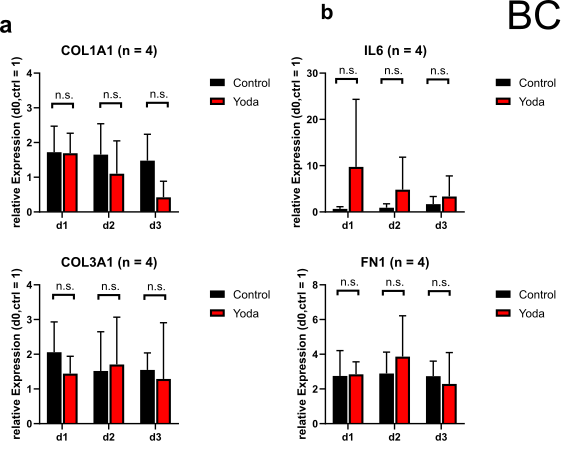
\includegraphics[scale = 0.6]{Collection.png}
    \caption{
    PCR Experiments where we saw some really cool stuff happening. 
    \textbf{a}: Col1$\alpha$1 output \textit{(n = 4)}
    \textbf{b}: Interleukin 6 out \textit{(n=23445)}
    All Experiments had n = 4. 
    }
    \label{fig:my_label}
\end{figure}

\subsection{WesternBlot}

\subsection{qRT-PCR}

\section{Excursion: Biostability of Yoda1}
\label{sec:biostability}